\documentclass{article}

\usepackage[utf8]{inputenc}
\usepackage{enumitem}
\usepackage{latexsym}
\usepackage{amsfonts}
\usepackage{amsmath,amssymb,amsthm}
\usepackage{amsfonts}
\usepackage{parskip}
\usepackage{listings}

\usepackage{xcolor}
\usepackage{multicol}

\usepackage{tikz}
\usetikzlibrary{arrows, automata, bending, positioning}

\newcommand{\set}[1]{\{#1\}}
\newcommand{\Z}{\mathbb{Z}}
\renewcommand{\epsilon}{\varepsilon}

\newenvironment{question}[2]
{
    {\large \textbf{Question #1.}}\\
    #2 \newline\newline
    \textbf{Answer:}
}{}{\newpage}

\title{Midterm 2}
\author{Asier Garcia Ruiz}

\begin{document}
\maketitle

\begin{question}
    {0}
    {Honor Code}
    I commit to uphold the ideals of honor and integrity by refusing to betray the trust bestowed upon me as a member of the Georgia Tech community.
    Signature: Asier Garcia Ruiz
\end{question}

\begin{question}
    {1a}
    {(2 points) Let $L$ = $\{w \in \{a,b,c,d\}^* \ |\ w$ has an equal number of
        $a$'s and $b$'s, and an equal number of $c$'s and $d$'s $\}$. You want to use the
        pumping lemma to show $L$ is not context-free. You have already assumed $L$ is
        context-free, and set $p$ to be the pumping length for $L$. Which, if any, of the
        following strings can you choose for the string $s$ that is pumped and leads to a
        contradiction? (Circle all that apply. No explanation needed.)

        \begin{multicols}{2}
            \begin{itemize}
                \item $abcd$
                \item $a^pb^pc^pd^p$
                \item $(abcd)^p$
                \item $a^pcb^pd$
            \end{itemize}
        \end{multicols}
        \
    }

    $a^pcb^pd$, $a^pb^pc^pd^p$
\end{question}

\begin{question}
    {1b}
    {(2 points) Let $G$ be a context free grammar with one nonterminal and $n$
        rules. If $G$ generates a finite number of words, what is the maximum possible
        number of words generated by $G$? Defend your answer.}
    We have that $G$ generates only a finite amount of words. This implies there are no rules of the form $A \to A$, as this would imply
    we can generate an infinite number of words by simply repeating this rule. We also cannot have something like $A \to B, B \to A$ as this
    would again imply we can make an infinite amount of words. Therefore, We cannot have any nonterminal symbols on the RHS of any rule.
    Because $G$ only has one nonterminal, it must be on the left the side, and the $n$ rules contain all the terminals. The maximum possible
    number of words generated by $G$ is thus the maximum length of the rules on the right side.
\end{question}

\begin{question}
    {1c}
    {(2 points) Here is a claim, and an attempted proof of the claim. Find the
        error in the proof (do not worry about whether the claim is true):
        \textit{\underline{Claim:} For any context free grammar $G$ generating $L$
            containing at least 2 non-terminals, you can construct a grammar $G'$ for $L$ such
            that $G'$ has one fewer non-terminal than $G$. \\\\
            ``Proof": ``Pick a non-terminal, non-start symbol A from G. Let $A \rightarrow w_1
                | ... | w_n$ be all the rules of $G$ with $A$ on the left hand side. Delete these
            rules. Then replace each rule of the form $X \rightarrow uAv$ with the rules $X \
                rightarrow uw_1v | ... | uw_nv$.  This grammar generates the same language as $G$,
            but it has one less non-terminal, since it doesn't contain $A$. Q.E.D." }}

    Consider our answer for 2b. We have the CFG
    \begin{align*}
        S & \to 0S0|A        \\
        A & \to 1B1          \\
        B & \to 0B0|\epsilon \\
    \end{align*}

    Getting rid of the nonterminal $B$ and applying the transformation would result in the following grammar
    \begin{align*}
        S & \to 0S0|A      \\
        A & \to 10A01|1001 \\
    \end{align*}
    This grammar does not produce the same strings as the original grammar as now the recursion produces $10A01$ instead of
    $0B0$.

    The error in the proof occurs when we allow the deletion of of nonterminals that have nonterminals on the left hand side.
    This makes it so the recursion cannot act the same way and creates issues like the one exemplified above.

\end{question}

\begin{question}
    {2a}
    {Give a CFG for each of the following languages: $L_1 = \{a^ib^jc^kd^l\ |\ i+j = k+l, i,j,k,l \geq 0$ are
        integers$\}$}

    We can use this CFG
    \begin{align*}
        S   & \to A | B          \\
        A   & \to aAd | C_1      \\
        C_1 & \to  bC_1d | D_1   \\
        D_1 & \to bD_1c|\epsilon \\
        B   & \to aBd | C_2      \\
        C_2 & \to  aC_1c | D_2   \\
        D_2 & \to bD_2c|\epsilon \\
    \end{align*}
\end{question}

\begin{question}
    {2b}
    {Give a CFG for each of the following languages: $L_2 = \{ ww^R\ |\ w$ is a binary string and contains exactly one $1$$\}$, $w^R$ is the reverse of $w$.}
    \begin{align*}
        S & \to 0S0|A        \\
        A & \to 1B1          \\
        B & \to 0B0|\epsilon \\
    \end{align*}
\end{question}

\begin{question}
    {3a}
    {Give a state diagram for the PDA recognizing $L_1$ from problem 2.}

    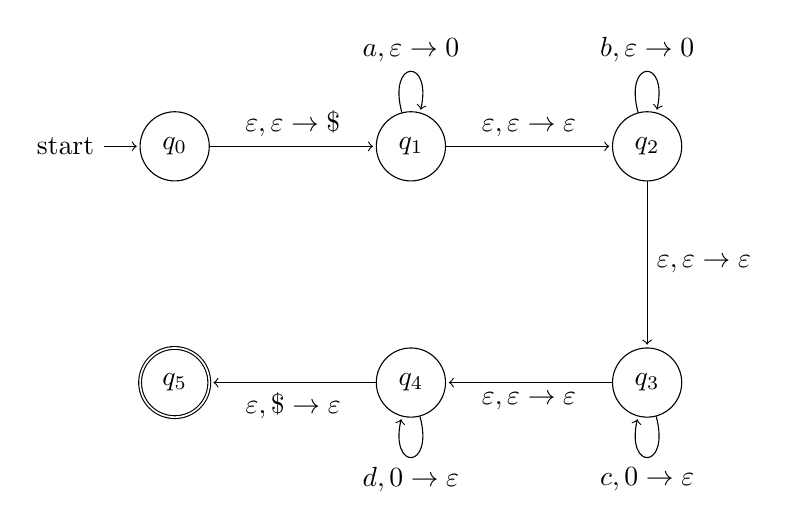
\begin{tikzpicture}[shorten >=1pt,node distance=3cm,on grid,auto]
        \node[state, initial]       (q_0)                                  {$q_0$};
        \node[state]                (q_1)    [right of=q_0]                {$q_1$};
        \node[state]                (q_2)    [right of=q_1]                {$q_2$};
        \node[state]                (q_3)    [below of=q_2]                {$q_3$};
        \node[state]                (q_4)    [left of=q_3]                {$q_4$};
        \node[state, accepting]     (q_5)    [left of=q_4]                {$q_5$};

        \path[->]   (q_0) edge node {$\epsilon, \epsilon \to \$$} (q_1)
        (q_1) edge [loop above] node {$a, \epsilon \to 0$} ()
        edge node {$\epsilon, \epsilon \to \epsilon$} (q_2)
        (q_2) edge [loop above] node {$b, \epsilon \to 0$} ()
        edge node {$\epsilon, \epsilon \to \epsilon$} (q_3)
        (q_3) edge [loop below] node {$c, 0 \to \epsilon$} ()
        edge node {$\epsilon, \epsilon \to \epsilon$} (q_4)
        (q_4) edge [loop below] node {$d, 0 \to \epsilon$} ()
        edge node {$\epsilon, \$ \to \epsilon$} (q_5)
        ;
    \end{tikzpicture}
\end{question}

\begin{question}
    {3b}
    {Give a state diagram for the PDA recognizing $L_2$ from problem 2.}
    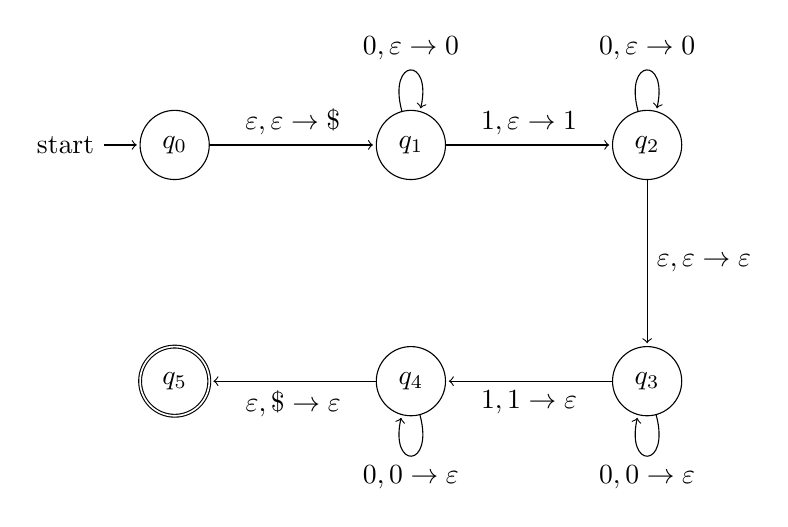
\begin{tikzpicture}[shorten >=1pt,node distance=3cm,on grid,auto]
        \node[state, initial]       (q_0)                                  {$q_0$};
        \node[state]                (q_1)    [right of=q_0]                {$q_1$};
        \node[state]                (q_2)    [right of=q_1]                {$q_2$};
        \node[state]                (q_3)    [below of=q_2]                {$q_3$};
        \node[state]                (q_4)    [left of=q_3]                {$q_4$};
        \node[state, accepting]     (q_5)    [left of=q_4]                {$q_5$};

        \path[->]   (q_0) edge node {$\epsilon, \epsilon \to \$$} (q_1)
        (q_1) edge [loop above] node {$0, \epsilon \to 0$} ()
        edge node {$1, \epsilon \to 1$} (q_2)
        (q_2) edge [loop above] node {$0, \epsilon \to 0$} ()
        edge node {$\epsilon, \epsilon \to \epsilon$} (q_3)
        (q_3) edge [loop below] node {$0, 0 \to \epsilon$} ()
        edge node {$1, 1 \to \epsilon$} (q_4)
        (q_4) edge [loop below] node {$0, 0 \to \epsilon$} ()
        edge node {$\epsilon, \$ \to \epsilon$} (q_5)
        ;
    \end{tikzpicture}
\end{question}

\begin{question}
    {4}
    {Prove that $L_3$ = $\{ww^R1^n ~|~ w$ is a binary string with $n$ $1$'s $\}$ is not context-free.\\
        Here is an example string from this language: \textcolor{red}{011}\textcolor{blue}{110}11.  Note that \textcolor{red}{011}\textcolor{blue}{110}111
        is not a string of the language.}

    Assume, for the sake of contradiction, that $L_3$ is context-free. Take $p$ to be pumping length. Now, consider the string
    $z = 0^p1^{2p}0^p1^p \in L_3$. Clearly we see that $|z| > p$, we know by the pumping lemma that there exist $u, v, x y z$ such that
    $z = uvxyz$, $|vxy| \leq p|$, and $|vy| > 0$. Since $L_3$ is context free (by our assumption), we also have that $uv^ixy^iz \in L_3$ for all
    $i \geq 0$.

    Now consider the following cases for what $vxy$ contains.

    \textbf{Case 1:} $vxy$ contains only 0s.\\
    If this is the case, then letting $i = 2$ we see that $uv^2xy^2z \not \in L_3$ since $w \neq (w^R)^R$ as one of them will have more 0s, a contradiction.

    \textbf{Case 2:} $vxy$ contains only 1s.\\
    If this is the case, then letting $i = 2$ we see that $uv^2xy^2z \not \in L_3$. Consider the case where $vxy$ only contains 1s from the $1^n$ segment,
    then the number of 1s at the end will be greater than the number of 1s withing $w$ and $w^R$. Now consider the case where $vxy$ contains 1s from the
    $w$ or $w^R$ segment, then the number of 1s in this segment will be greater than the number of 1s in the $1^n$ segment. Both of these lead to a
    contradiction.

    \textbf{Case 3:} $vy$ contains 0s followed by 1s.\\
    In this case then, then letting $i = 2$ we have that $uv^2xy^2z \not \in L_3$ because $w$ will not equal $(w^R)^R$ as there will be more 0s in either
    $w$ or $w^R$. This is a contradiction.

    \textbf{Case 4:} $vy$ contains 1s followed by 0s.\\
    In this case then, then letting $i = 2$ we have that $uv^2xy^2z \not \in L_3$ because $w$ will not equal $(w^R)^R$ as there will be more 0s in either
    $w$ or $w^R$. This is a contradiction.

    Therefore, since we have encountered contradictions in all scenarios, we have that $L_3$ is not a context-free grammar.
\end{question}
\end{document}